\documentclass{article}

% Language setting
% Replace `english' with e.g. `spanish' to change the document language
\usepackage[spanish,mexico]{babel}

% Set page size and margins
% Replace `letterpaper' with `a4paper' for UK/EU standard size
\usepackage[letterpaper,top=2cm,bottom=2cm,left=3cm,right=3cm,marginparwidth=1.75cm]{geometry}

% Useful packages
\usepackage{amsmath}
\usepackage{graphicx}
\usepackage[colorlinks=true, allcolors=blue]{hyperref}

\title{Propuesta de investigación}
\author{Erick Felipe Serrato Garcia}

\begin{document}
\maketitle

\begin{abstract}
Here is the abstract
\end{abstract}

\section{Introducción}

El cancer es uno de los temas médicos más relevantes en la actualidad debido al riesgo que este presenta en todos los sectores de la población, en caso de que no se detecte a tiempo puede llegar a ser muy dificil de tratar e inclusive solo dar tratamiento para extender la vida del paciente un poco más.

Cuando una célula envejece y pierde su capacidad de dividirse termina su ciclo de vida, las células cancerígenas son células anomalas que presentan mutaciones en los genes que regulan el ciclo celular, por ello pueden crecer descontroladamente hasta formar densidades grandes de ellas y posteriormente diseminarse a otras partes del cuerpo.

El cuerpo humano puede defenderse de diferentes amenazas, desde las que ingresan del exterior hasta las que se producen en el interior, en el caso de las células cancerigenas, si el cuerpo humano se encuentra saludable (entre otros factores) puede erradicar y/o contener la enfermedad. A la interacción en la que las células defensoras eliminan a las anomalas se le llama citotoxicidad.

Cuando el sistema inmune detecta una anomalía, envia a las células llamadas "natural killers" que es un tipo de glóbulo blanco que puede matar células tumorales, células infectadas por virus o cualquier cosa que consideren anomala, estas no siempre tienen exito en su misión, cuando eso sucede, el sistema inmune envía a los lifocitos T o células T las cuales identifican a las células infectadas y las eliminan mediante un proceso llamado aptosis y posteriormente otras células "limpiadoras" llamadas macrofagos terminan de limpiar los restos.

\subsection{Efecto Allee en poblaciones de células}


Los modelos tradicionales para poblaciones de cáncer consideran que crece de manera exponencial, limitado por los nutrientes y el espacio disponible, sin embargo estudios clínicos recientes muestran que el crecimiento puede comportarse como una dinámica con efecto Allee dependiendo la densidad de población que se tenga\cite{Gerlee032022}.

La interacción entre células defensoras y cancerigenas puede explicarse de manera general como una dinámica de poblaciones entre presas y predadores, en la naturaleza si una densidad de población es demasiado baja y continua bajando se tiene una tasa de crecimiento negativa, tenemos otro caso en el cual la tasa de crecimiento es baja pero positiva, esto puede ser modelado mediante el efecto Allee fuerte y débil respectivamente, esto podemos visualizarlo en la Figura \ref{fig:allees}.


\begin{figure}[ht]
    \centering
    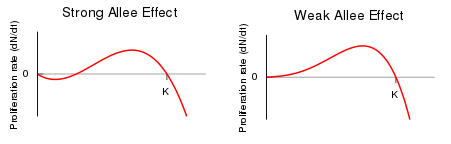
\includegraphics[width=0.6\textwidth]{images/Allee.png}
    \caption{Efecto Allee débil y fuerte}
    \label{fig:allees}
\end{figure}

En el efecto Allee débil (ecuación \ref{eqn:weak_allee}) la tasa de crecimiento aumenta con la densidad de población y permanece positiva, en el efecto fuerte \ref{eqn:strong_allee}, se tiene un umbral poblacional por debajo del cual la población decrece hasta llegar a la extinción.

\begin{equation}
    \frac{d x}{ dt} = r x (1 - \frac{x}{k})(1- \frac{A+ c}{x + c})
    \label{eqn:strong_allee}
\end{equation}

El caso débil es cuando $A\leq 0$, si consideramos $A=0$ y se obtiene:

\begin{equation}
    \frac{d x}{ dt} = r x (1 - \frac{x}{k})(\frac{x}{x + c})
    \label{eqn:weak_allee}
\end{equation}

La finalidad del presente es tratar de modificar el tratamiento de dosis máxima tolerada por una terapia mediante la predicción y control de densidades poblacionales cancerigenas, ya que al utilizar constantemente las dosis máximas toleradas se daña de manera simultanea al cancer y al cuerpo humano.


\subsection{Complejo MHC y su importancia en el cancer}
Como hemos discutidos los linfocitos y natural killers atacan a los antígenos, la diferencia es que las natural killers atacan a lo que consideren anomalo y los  linfocitos ya tienen identicadas a las células que deben destruir, esto es debido a que las células infectadas ya están marcadas y esto es gracias al complejo principal de histocompatibilidad (MHC) el cual es una especie de "receptor" que se activa en las células infectadas poniendoles un identificador, con esto los linfocitos ya saben a que células destruir (Fígura \ref{fig:mhc}).

\begin{figure}[ht]
    \centering
    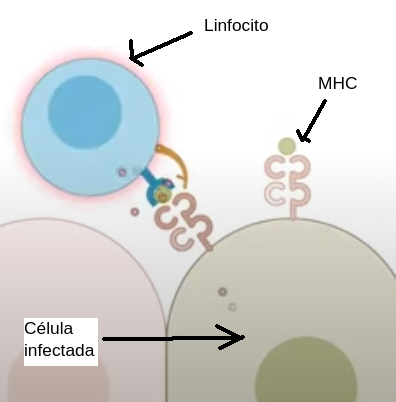
\includegraphics[width=0.4\textwidth]{images/mhc.png}
    \caption{Interacción de los linfocitos y células infectadas mediante el complejo MHC}
    \label{fig:mhc}
\end{figure}

El problema del crecimiento aberrante en la densidad de células cancerígenas es que las células infectadas pierden la capacidad de activar el MHC, por lo que no pueden ser identificadas y por lo tanto destruidas. En este punto nos preguntamos ¿si pudiesemos controlar la regulación del MHC disminuiría la densidad de células cancerigenas? la respuesta es que si. Existen diversos tratamientos aprobados por la FDA que promueven la regulación del THC y con ello aumentar la citotoxicidad de los linfocitos en las células cancerigenas \cite{Cornel072020}. Esto último nos lleva a considerar la regulación del THC como una variable a controlar que entre mayor sea se verá una disminución en la densidad de población de células cancerigenas.


 \newpage
\section{Problema propuesto}
Como explicamos en la sección 1.1, si se detecta a tiempo, las celulas cancerigenas no tienen un crecimiento exponencial, esto debido a que las celulas defensoras del cuerpo humano compiten con las células cancerigenas para aniquilarlas, es decir, se comportan como presas y depredadores, dicho esto, veamos la figura \ref{fig:case_1}, tenemos dos dominios, el dominio con la especie de color azul (farmaco) y el dominio en donde se encuentran las especies de celulas cancerigenas (rojo) y celulas defensoras del cuerpo humano (verde).

Inicialmente interactuan las celulas cancerigenas con las celulas del cuerpo humano compitiendo entre sí, las celulas defensoras predando a las celulas cancerigenas, a esto lo consideramos el primer caso:
\begin{figure}[ht]
    \centering
    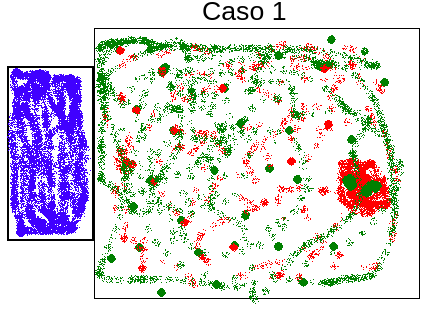
\includegraphics[width=0.5\textwidth]{images/caso1.png}
    \caption{Caso 1}
    \label{fig:case_1}
\end{figure}
En el caso 1 tenemos un sistema reacción difusión

Como suele suceder, las especie cancerigena crece demasiado rápido por lo que no bastan las celulas defensoras para contenerlo por ello se administran medicamentos, a esto llamamos el caso 2 (figura \ref{fig:case_2}).
En el caso 2, el dominio en donde se encuentra el medicamento (azul), fluye desde su espacio hacia donde se encuentran las especies defensoras y cancerigenas cooperando con las celulas defensoras para aniquilar a las cancerigenas.

En el caso 2 podemos considerar la dinámica de dominios estratificados en sistemas reacción difusión con 3 especies.

\begin{figure}[ht]
    \centering
    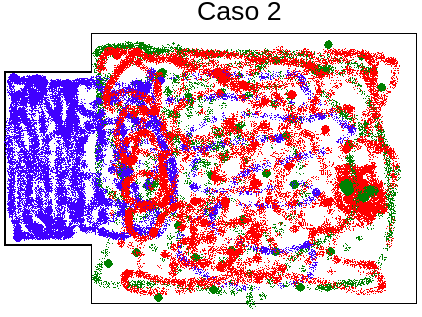
\includegraphics[width=0.5\textwidth]{images/caso2.png}
    \caption{Caso 2}
    \label{fig:case_2}
\end{figure}


Como ya es bien sabido por la comunidad científica, cuando el cancer crece demasiado suele migrar a diferentes partes del cuerpo, este fenomeno es conocido como metastais.

En el caso 3 consideramos que las celulas cancerigenas ya crecieron tanto que el sitio en donde se encontraba (color rojo en figura \ref{fig:case_3}) se ha convertido en una fuente que va a incorporarse a un sistema de tuberias para poder llegar a mas sitios, estas tuberias ya tienen por defecto un flujo constante que arrastrará a la especie cancerigena, consideremos también que tenemos dentro del flujo a las defensas del cuerpo (color verde) y a su vez se administrará medicamento (azul) desde diferentes sitios con el fin de aniquilar a las celulas cancerigenas. 

\begin{figure}[ht]
    \centering
    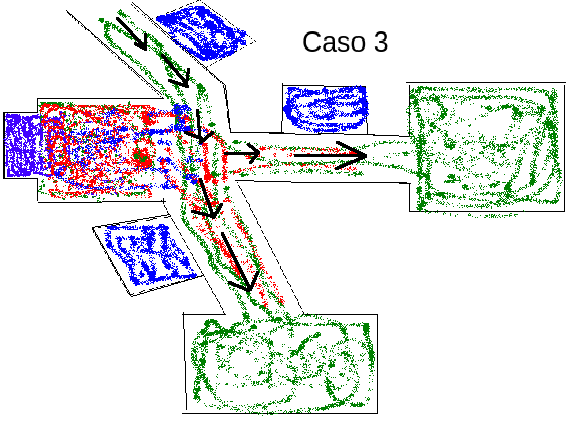
\includegraphics[width=0.5\textwidth]{images/caso3.png}
    \caption{Caso 3}
    \label{fig:case_3}
\end{figure}

Tengamos en cuenta que los pacientes tienen dosis máxima tolerada, el fin de este trabajo es estudiar en que casos es necesario administrar dosis máximas y en que casos necesitamos plantear una logística para administrar el medicamento que coopere con las defensas del cuerpo con el fín de mantener al mínimo o inclusive aniquilar a las celulas cancerigenas.


\section{Modelo propuesto}

Consideremos un entorno en el cual interactuan 3 especies, el cancer, células sanas y el sistema inmune. Sabemos que el cancer compite por los recursos y el espacio con las células sanas, por otra parte el sistema inmune si caza a a las células cangerigenas, por ello consideremos la siguiente matriz de interacción:

\begin{equation}
    \begin{pmatrix}
       r_c C (\frac{C}{a} - 1)(1-\frac{C}{k_c}) & -\alpha CS & -\beta CI \\ \\
    -\gamma CS & r_s S (1 - \frac{S}{k_s}) & \delta SI \\ \\
    \eta C I & 0 & r_i I(1-\frac{I}{k_i})
    \end{pmatrix}
    \label{eqn:matriz_interaccion}
\end{equation}
 
En donde   $C$ es el cancer, $S$ son las células sanas e $I$ es el sistema inmune, con ello podemos escribir el siguiente sistema de ecuaciones diferenciales ordinarias:

\begin{equation}
    \frac{dC}{dt} =  r_c C (\frac{C}{a} - 1)(1-\frac{C}{k_c}) - \alpha CS - \beta CI,
    \label{eqn:cancer_dynamic}
\end{equation}

\begin{equation}
    \frac{dS}{dt} = r_s S (1 - \frac{S}{k_s})  - \gamma CS + \delta SI,
    \label{eqn:sano_dynamic}
\end{equation}


\begin{equation}
    \frac{dI}{dt} = r_i I(1-\frac{I}{k_i}) + \eta C I.
    \label{eqn:inmune_dynamic}
\end{equation}


Analizando los elementos de la diagonal de le ecuacion \ref{eqn:matriz_interaccion} consideremos el término asociado el cancer $C$ mediante el modelo del efecto Allee efecto Allee $g(C) = r_c C (\frac{C}{a} - 1)(1-\frac{C}{k_c})$, en donde $0<h<r$ corresponde al efecto Allee fuerte y $r<0$,  $h>0>r$ es el efecto débil y que al ser una ecuación cúbica tiene valores nulos para $C=0$, $C=r$ y $C=h$, podemos visualizar las curvas en la figura \ref{fig:allee_plots}

\begin{figure}[ht]
 \centering
  {
   \label{fig:strong_allee}
a)    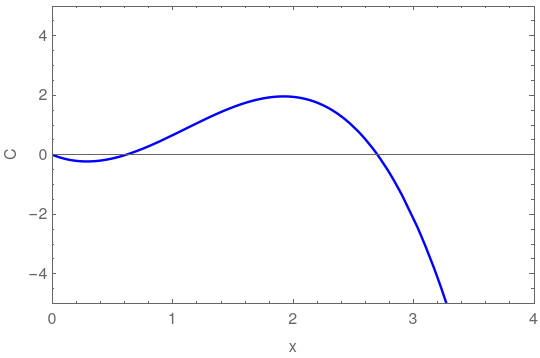
\includegraphics[width=0.45\textwidth]{images/strong_allee.png}}
  {
   \label{fig:weak_allee}
b)    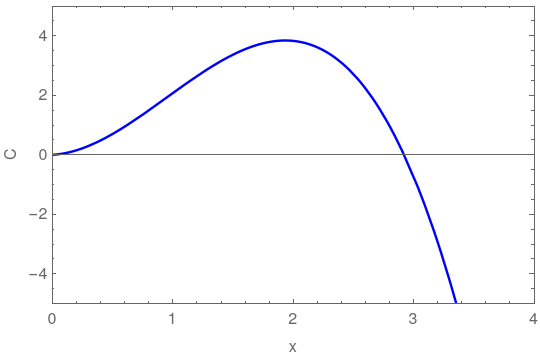
\includegraphics[width=0.45\textwidth]{images/allee_weak.png}}
  
 \caption{En $a)$ tenemos el efecto Alle fuerte para $r=2.7$ y $h=0.61$, en $b)$ tenemos el efecto débil con $r=-0.08$ y $h=2.92$}
 \label{fig:allee_plots}
\end{figure}


Para el caso de las células sanas $S$, consideramos un modelo logístico $r_s S (1 - \frac{S}{k_s})$. 

Para el sistema inmune $S$, consideramos un modelo logístico $r_i I(1-\frac{I}{k_i})$, este tiene valores nulos cuando $I=0$ y cuando $I=k_i$ es en donde la cantidad de individuos tiende a un valor constante.

\begin{figure}[ht]
    \centering
    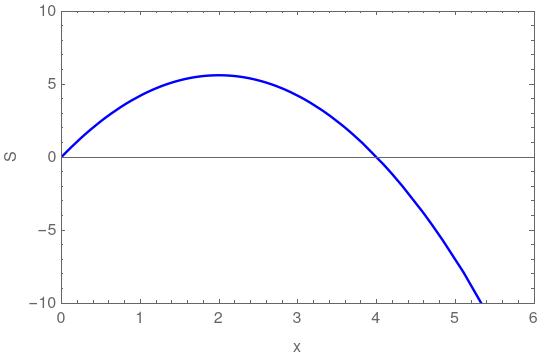
\includegraphics[width=0.5\textwidth]{images/logistic.png}
    \caption{Modelo logístico que modela la producción de céluas inmunitarias $S$, con $r_i=5.6 $ y $k_i=4$}
    \label{fig:logistic}
\end{figure}

\subsection{Escalamiento de EDP}
De las ecuaciones \ref{eqn:cancer_dynamic}, \ref{eqn:sano_dynamic}, \ref{eqn:inmune_dynamic} consideremos el cambio de variable $c=\frac{C}{k_c}$,  $s=\frac{S}{k_s}$, $i=\frac{I}{k_i}$ y $t = \frac{a}{k_c r_c} \tau $ resolviendo obtenemos:

\begin{equation}
    \frac{dc}{d \tau} =  c (c - a')(1-c) - \alpha' cs - \beta' i c,
    \label{eqn:cancer_dynamic_escalado}
\end{equation}

\begin{equation}
    \frac{ds}{d \tau} = r_s ' s (1 - s)  - \gamma' cs + \delta' si,
    \label{eqn:sano_dynamic_escalado}
\end{equation}


\begin{equation}
    \frac{di}{d\tau} = r_i ' i(1-i) + \eta' ci.
    \label{eqn:inmune_dynamic_escalado}
\end{equation}

En donde $a' = \frac{a}{k_c}$, $\alpha'= \alpha k_s$, $\beta'=\beta k_i$, $r_s'= \frac{a r_s}{k_c r_c}$, $\gamma'=\frac{a \gamma}{r_c}$, $\delta' = \frac{a \delta}{r_c k_c}$, $r_i' = \frac{a r_i}{r_c k_c}$ y $\eta' = \frac{a \eta}{r_c k_c}$

\subsection{Estados estacionarios y nulclinas test}

Los estados estacionarios se encuentran cuando se cumple que las ecuaciones \ref{eqn:cancer_dynamic_escalado}, \ref{eqn:sano_dynamic_escalado} y \ref{eqn:inmune_dynamic_escalado} no varian temporal ni espacialmente, es decir:

\begin{equation}
    c (c - a')(1-c) - \alpha' cs - \beta' i c = 0,
    \label{eqn:cancer_dynamic_escalado_2}
\end{equation}

\begin{equation}
     s (1 - s)  - \gamma'' cs + \delta'' si = 0,
    \label{eqn:sano_dynamic_escalado_2}
\end{equation}


\begin{equation}
    i(1-i) + \eta'' ci = 0.
    \label{eqn:inmune_dynamic_escalado_2}
\end{equation}

En donde $\gamma'' = \frac{\gamma k_c}{r_s}$,  $\delta'' = \frac{\delta}{r_s}$ y $\eta'' = \frac{\eta}{r_i}$,  las ecuaciones \ref{eqn:cancer_dynamic_escalado_2}, \ref{eqn:sano_dynamic_escalado_2} y \ref{eqn:inmune_dynamic_escalado_2} se cumplen cuando $c=0$, $s=0$ e $i=0$ y cuando 

\begin{equation}
    (c - a')(1-c) - \alpha' s - \beta' i  = 0,
    \label{eqn:cancer_dynamic_escalado_3}
\end{equation}

\begin{equation}
    (1 - s)  - \gamma'' c + \delta'' i = 0,
    \label{eqn:sano_dynamic_escalado_3}
\end{equation}


\begin{equation}
    (1-i) + \eta'' c = 0.
    \label{eqn:inmune_dynamic_escalado_3}
\end{equation}

de la ecuación  \ref{eqn:inmune_dynamic_escalado_3} podemos despejar

\begin{equation}
    c =  \frac{ i-1}{\eta},
    \label{eqn:inmune_dynamic_escalado_4}
\end{equation}

Sustituyendo \ref{eqn:inmune_dynamic_escalado_4} en \ref{eqn:cancer_dynamic_escalado_3} y despejando tendremos:

\begin{equation}
 F_1 (s,i) = -s \alpha' - i\beta' - \frac{(-1+i-\eta'')(-1+i -a \eta'')}{(\eta'')^2}  = 0
    \label{eqn:sol_s1}
\end{equation}


De la ecuación \ref{eqn:sol_s1} despejamos a $s$ lo que nos dá:

\begin{equation}
    s_a(i) = -\frac{a' (\eta'') ^2+a' \eta'' +\eta'' +1}{\alpha'  (\eta'') ^2}+\frac{ \left(a' \eta'' -\beta'  (\eta'') ^2+\eta''
   +2\right)}{\alpha'  (\eta'') ^2}i-\frac{i^2}{\alpha'  (\eta'') ^2}
   \label{eqn:sol_s11}
\end{equation}


Sustituyendo \ref{eqn:inmune_dynamic_escalado_4} en \ref{eqn:sano_dynamic_escalado_3} y despejando tendremos:

\begin{equation}
    F2(s,i) = -\delta''  i-\frac{\gamma''  (i-1)}{\eta }-s+1 = 0
    \label{eqn:sol_s22}
\end{equation}

y nuevamente, despejando a $s$, tenemos:

\begin{equation}
    s_b(i) = -\frac{i (\gamma'' +\delta''  \eta'' )}{\eta'' }+\frac{\eta'' +\gamma''  }{\eta'' }
    \label{eqn:sol_s2}
\end{equation}


para la intersección, en ambos casos debe cumplirse que $s_1=s_2$, resolviendo para $i$ tenemos dos soluciones:

\tiny{
\begin{multline}
i_1 =\frac{1}{2}(\eta''  \sqrt{(\alpha') ^2 (\gamma'' +\delta''  \eta'' )^2+(a')^2+2 a' (\alpha'  (\gamma'' +\delta''  \eta'' )-\beta'  \eta'' -1)-2 \alpha' 
   \left(\gamma''  (\beta'  \eta'' -1)+\delta''  \left(\beta'  (\eta'') ^2-\eta'' -2\right)+2\right)+  (\beta')^2 (\eta'') ^2-2 \beta'  \eta'' -4 \beta'
   +1} \\ +\alpha'  \gamma''  \eta'' +\alpha'  \delta'  (\eta'') ^2+a' \eta'' -\beta'  (\eta'' )^2+\eta'' +2 )
  \label{eqn_sol_i1}
\end{multline}
}

\tiny{
\begin{multline}
i_2 = \frac{1}{2}(-\eta''  \sqrt{(\alpha') ^2 (\gamma'' +\delta''  \eta'' )^2+(a')^2+2 a' (\alpha'  (\gamma'' +\delta''  \eta'' )-\beta'  \eta'' -1)-2 \alpha' 
   \left(\gamma''  (\beta'  \eta'' -1)+\delta''  \left(\beta'  (\eta'') ^2-\eta'' -2\right)+2\right)+  (\beta')^2 (\eta'') ^2-2 \beta'  \eta'' -4 \beta'
   +1} \\ +\alpha'  \gamma''  \eta'' +\alpha'  \delta'  (\eta'') ^2+a' \eta'' -\beta'  (\eta'' )^2+\eta'' +2 )
  \label{eqn_sol_i2}
\end{multline}
}
\normalsize
Retomando, buscamos que se satisfasgan las ecuaciones \ref{eqn:cancer_dynamic_escalado_3}, \ref{eqn:sano_dynamic_escalado_3} y \ref{eqn:inmune_dynamic_escalado_3}, al sustituir  en ellas \ref{eqn:inmune_dynamic_escalado_4} se obtienen las ecuaciones \ref{eqn:sol_s1} y \ref{eqn:sol_s22}, que solo depende de $s$ e $i$, sabemos la solución se encuentra en dos puntos al encontrar $i_1$ e $i_2$:

\begin{equation}
   P_1 = (i_1, c_1, s_1)    
\end{equation}

\begin{equation}
    P_2 = (i_2, c_2, s_2)
\end{equation}

La intersección en las ecuaciones \ref{eqn:sol_s1} y \ref{eqn:sol_s22} pueden tener valores positivos y negativos, sin embargo, las densidades de población no tienen sentido para valores negativos por lo que además de buscar los puntos $P_1$ y $P_2$, también debe cumplirse que sean positivos, en la figura \ref{fig:nullclines} podemos observar algunos de los valores para los parámetros los cuales se cumplen estas condiciones.

\begin{figure}[ht]
    \centering
    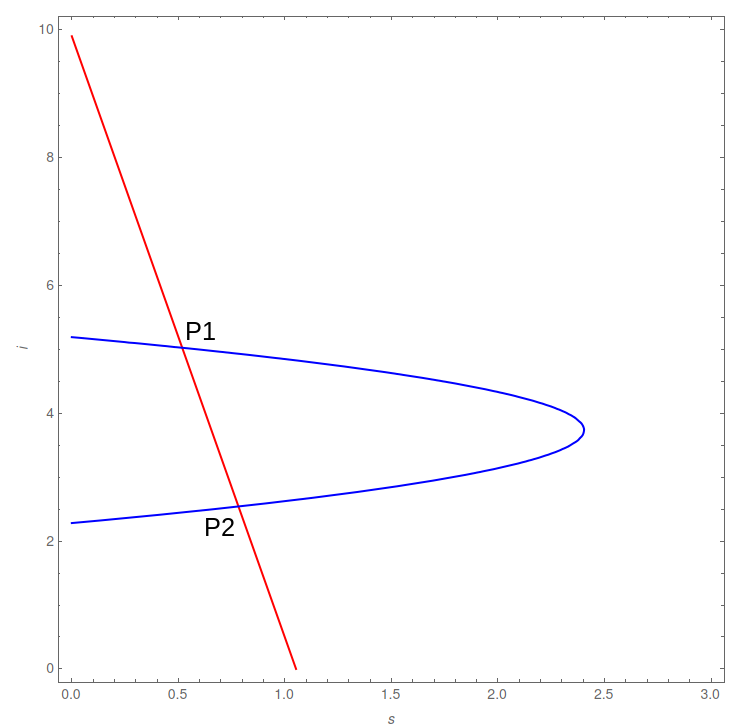
\includegraphics[width=0.4\textwidth]{images/nullclines.png}
    \caption{Representación gráfica de las ecuaciones $F_1(s,i)$ (azul) y $F_2(s,i)$ (rojo), para los valor es de $a'=6.24$, $\alpha'=1.19$, $\beta'=1.02$, $\gamma''=0.045$, $\delta''=0.054$, $\eta''=0.86$ con $P_1(i,c,s)=(5.024, 4.679, 0.518)$ y $P_2(i,c,s)=(2.541,1.791, 0.782)$}
    \label{fig:nullclines}
\end{figure}


\newpage
\subsection{Analisis de estabilidad lineal}

Ahora consideremos el sistema de ecuaciones \ref{eqn:cancer_dynamic_escalado}, \ref{eqn:sano_dynamic_escalado} y \ref{eqn:inmune_dynamic_escalado} con dependencia espacial

\begin{equation}
    \frac{\partial c}{\partial \tau} = D_c \nabla ^2 c +  c (c - a')(1-c) - \alpha' cs - \beta' i c,
    \label{eqn:cancer_dynamict_escalado}
\end{equation}

\begin{equation}
    \frac{\partial s}{\partial \tau} = D_s \nabla ^2 s + r_s ' s (1 - s)  - \gamma' cs + \delta' si,
    \label{eqn:sano_dynamict_escalado}
\end{equation}


\begin{equation}
    \frac{\partial i}{\partial \tau} = D_i \nabla ^2 i + r_i ' i(1-i) + \eta' ci.
    \label{eqn:inmune_dynamict_escalado}
\end{equation}
 
\newpage
\bibliographystyle{alpha}
\bibliography{sample}

\end{document}